\documentclass{article}
\usepackage{pythonhighlight}
\usepackage{graphicx}
\usepackage{ctex}
\usepackage[left=3cm,top=3cm,right=3cm]{geometry}

% TITLE PAGE CONTENT %%%%%%%%%%%%%%%%%%%%%%%%
%%%%%%%%%%%%%%%%%%%%%%%%%%%%%%%%%%%%%%%%%%%%%
\newcommand{\labno}{02}
\newcommand{\labtitle}{EE208 Crawler}
\newcommand{\authorname}{Zhou Litao}
\newcommand{\studentno}{518030910407}
\newcommand{\classno}{F1803016}
% END TITLE PAGE CONTENT %%%%%%%%%%%%%%%%%%%%


\begin{document}

\begin{center}
{\LARGE \textsc{Laboratory No. \labno:} \\ \vspace{4pt}}
{\Large \textsc{\labtitle} \\ \vspace{4pt}} 
\rule[13pt]{\textwidth}{1pt} \\ \vspace{15pt}
{\large By: \authorname \\ \vspace{10pt}
No. \studentno \\ \vspace{10pt}
SJTU \classno \\ \vspace{10pt}
\today \vspace{20pt}}
\end{center}



\section{Introduction}

\subsection{Equipment}
\begin{itemize}
\item\textbf{Environment} Ubuntu 16.04 (on Virtual Machine)
\item\textbf{Language} Python 2.7.16 with packages as follows
	\begin{itemize}
	\item urllib 1.24.2
	\item beautifulsoup4 4.8.0
	\end{itemize}
\item\textbf{Tools} PyCharm 2019.2, Virtual Box
\end{itemize}
The Python script is also tested in Windows 10.

\subsection{Purpose}
In this experiment, there are three exercises for the construction of a crawler. First, we need to sign in the SJTU BBS and modify our self-introduction by means of POST requests. Second, we need to write a BFS function and return the graph structure as a crawling method. Finally, we should complete a simple crawler.

\subsection{Principle}
\label{sec:principle}
For the first exercise, the interactions we do with the website are in the form of requests (like GET, POST, etc.) in principle. So in order to manipulate our information board in SJTU BBS, all we need to do is to simulate a POST request in Python. This work can be easily implemented with the urllib module.

For the second and third exercise, a \textit{linear list} is used to store the vertices to be visited in the future. The linear list can be a stack, following the first-in-last-out rule, then the searching method will be DFS, since the closest vertex to the current vertex (which is also the latest added vertex) will be visited in the next step at once. The linear list can also be a queue, following the first-in-first-out rule, then the searching method will be BFS, since after the deeper vertices are added to the queue, they won't be visited until all the vertices above their levels have been visited. So with little modification to the given DFS function, we can write out a BFS function as the exercise requires.

For the fourth exercise, by combining the BFS or DFS program as we've written in exercise 2, all we have to do is to give concrete implementation of the get\_page() function and get\_all\_links() function. With urllib and BeautifulSoup parser, we can write out theses functions to complete a simple crawler.


\section{Procedure}
\subsection{Exercise 1}

\subsubsection{Solution}
In this exercise, our goal is to simulate a POST request to the SJTU BBS information board. As the Flowchart \ref{fig:flowchart} depicts, first we should put cookie into the urllib opener, so that the website can store our personal acoount information for further interaction. Then we input our username and password by means of POST request to login into our account. If the login succeeds, we can update our postdata on the personal information board page. With all the processes above finished, we can test whether our information has been indeed updated, as the end of the exercise program. As the flowchart shows, theses small steps have been well encapsulated into several functions, which will be explained in detail below.

\begin{figure}[htbp]
\centering
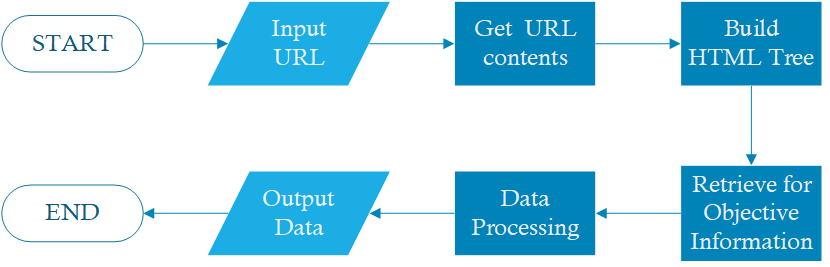
\includegraphics[width=9.5cm]{img/flowchart.png}
\label{fig:flowchart}
\caption{Flow Chart of the Exercise 1}
\end{figure}

\paragraph{BBS Login} To login the BBS, we need to first add cookie into our urllib opener, so that our input username and password can be recognized by the web server all the way through the experiment. The codes of this function have been provided in the tutorial, and encapsulated in a small function in my Python script.
\begin{python}
# bbs_set_sample.py
def bbs_init_cookie():
    cj = cookielib.CookieJar()      # 初始化cookie
    opener = urllib2.build_opener(urllib2.HTTPCookieProcessor(cj))
    urllib2.install_opener(opener)  # 将cookie加入opener
\end{python} 

Then we simulate a login POST request, sending our id and password to the server. By checking the actual POST request of SJTU BBS in Firefox, we know that the request-body is composed of three parts, namely, id, pw and submit. With the guidance of the tutorial, we write out the following login function.

\begin{python}
# bbs_set_sample.py
def bbs_login(id, pw):
    postdata = urllib.urlencode({    # 根据发出数据模拟request-body
        'id': id,
        'pw': pw,
        'submit': 'login'
    })
    req = urllib2.Request(url='https://bbs.sjtu.edu.cn/bbslogin', data=postdata)
    response = urllib2.urlopen(req)  # POST方式发出请求
    response = urllib2.urlopen('https://bbs.sjtu.edu.cn/bbsleftnew')  
                                  # 打开BBS欢迎页,查看ID是否显示在欢迎页中。
    return id in response.read()     # True则成功
\end{python}


\paragraph{Update Information}
After a successful login, we switch to the information board page. Still by checking the POST request format in Firefox, we know that the POST request here is composed of two elements, `type' and `test'. The structure of the function is similar to the login function. We return a bool value to check whether our updating is successful. A little difference here is that the success message in SJTU BBS is Chinese characters. We have to make sure that the web message matches our Python string in character encoding.

\begin{python}
def bbs_write(text):
    postdata = urllib.urlencode({    # 根据用户输入的text数据模拟request-body
        'type': 'update',
        'text': text
    })
    req = urllib2.Request(url='https://bbs.sjtu.edu.cn/bbsplan', data=postdata)
    response = urllib2.urlopen(req)  # 打开修改页,查看成功消息是否显示在修改页中。
    return "个人说明档修改成功。" in response.read().decode('gbk').encode('utf-8')
                                     # 将修改页重新编码,匹配成功消息
\end{python}

The functions above are combined in a \textit{bbs\_set} function as follows.
\begin{python}
# bbs_set_sample.py
def bbs_set(id, pw, text):
    bbs_init_cookie()
    if bbs_login(id, pw):
        if bbs_write(text):
            print "Write Success!"
        else:
            print "Write Failed!"
    else:
        print "Login Failed!"
    content = urllib2.urlopen('https://bbs.sjtu.edu.cn/bbsplan').read()
    soup = BeautifulSoup(content,features="html.parser")
    print str(soup.find('textarea').string).strip().decode('utf8')
\end{python}

\subsubsection{Results}
The test results can be found at graph \ref{img:1.1} and \ref{img:1.2}.

\begin{figure}[htbp]
\centering
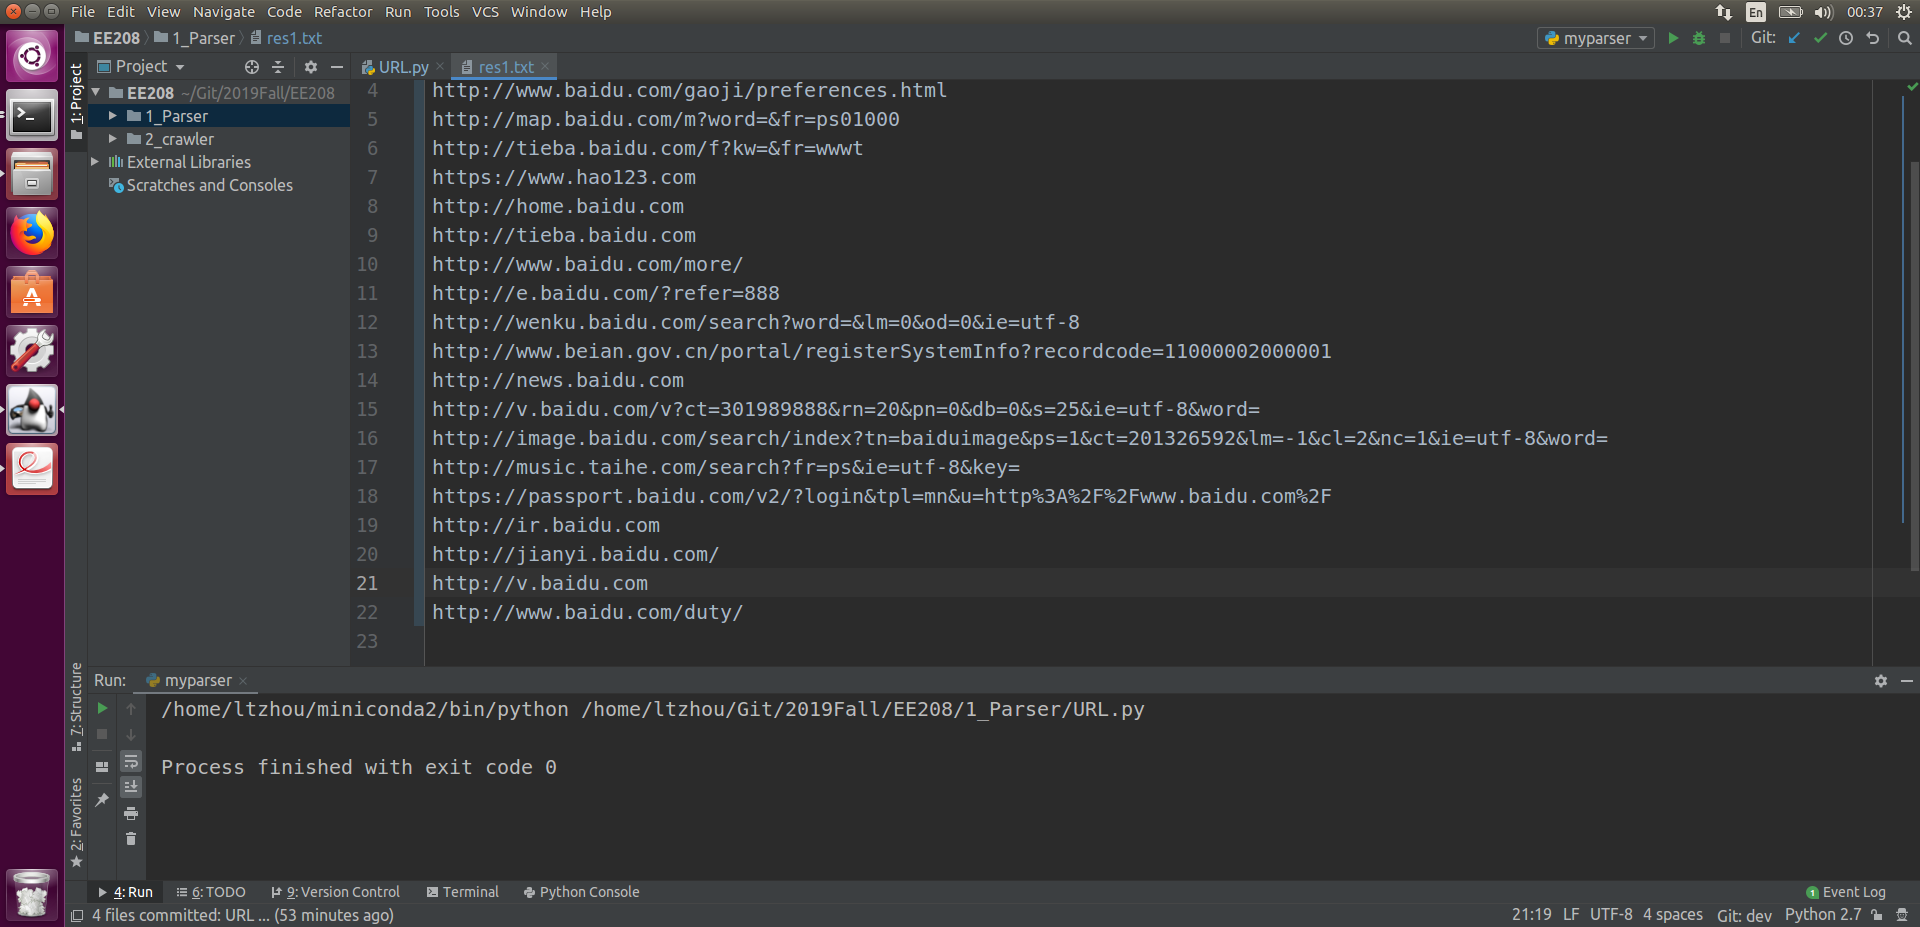
\includegraphics[width=9.5cm]{img/test1_1.png}
\caption{parseURL in PyCharm}
\label{img:1.1}
\end{figure}

\begin{figure}[htbp]
\centering
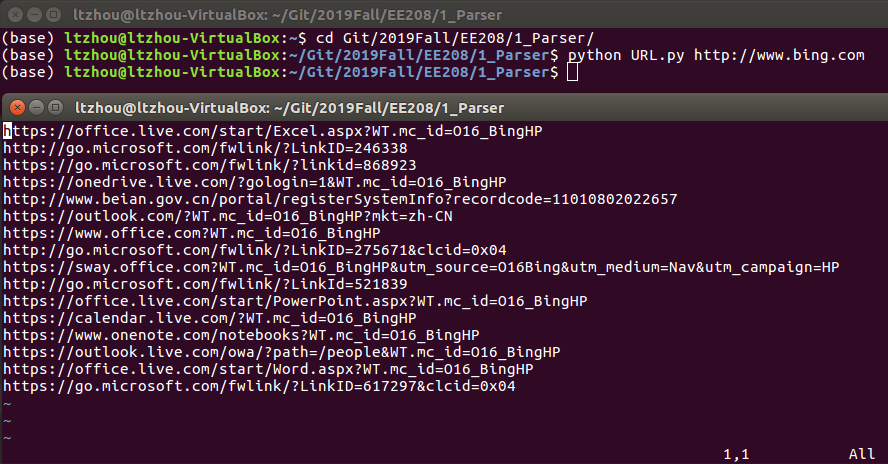
\includegraphics[width=9.5cm]{img/test1_2.png}
\caption{parseURL in console}
\label{img:1.2}
\end{figure}

\subsection{Exercise 2 \& 3}

\subsubsection{Solution}

In exercise 2, we should write a BFS function. As has been explained in the section \ref{sec:principle}, a little modification for the given DFS\_union function will make the job done. To be specific, we just change the `stack' structure into `queue' structure. The new elements should be added at the beginning of the list rather than the end. So we change the union function into the following codes, with the help of the list.insert() function. 

\begin{python}
# crawler_sample.py
def union_bfs(a,b):
    for e in b:
        if e not in a:
            a.insert(0,e)
\end{python}

In exercise 3, we should let our crawl() function return a graph structure, in the form of a (Parent node, list of ChildNode) dict. We note that when we are traversing through the graph, we automatically get the current node (page) and following nodes (outlinks), so we can just simply use a dict to record these data down. And since all the nodes will be visited exactly once, we can ensure the correctness of this method. The codes are listed below.

\begin{python}
# crawler_sample.py
while tocrawl:
    page = tocrawl.pop()
    if page not in crawled:        
    content = get_page(page)
        outlinks = get_all_links(content)
        graph[page] = outlinks  # the newly-added line for drafting a graph
        globals()['union_%s' % method](tocrawl, outlinks)
        crawled.append(page)
return graph, crawled
\end{python}


\subsubsection{Results}

The test results can be found at graph \ref{img:2.1} and \ref{img:2.2}.

\begin{figure}[htbp]
\centering
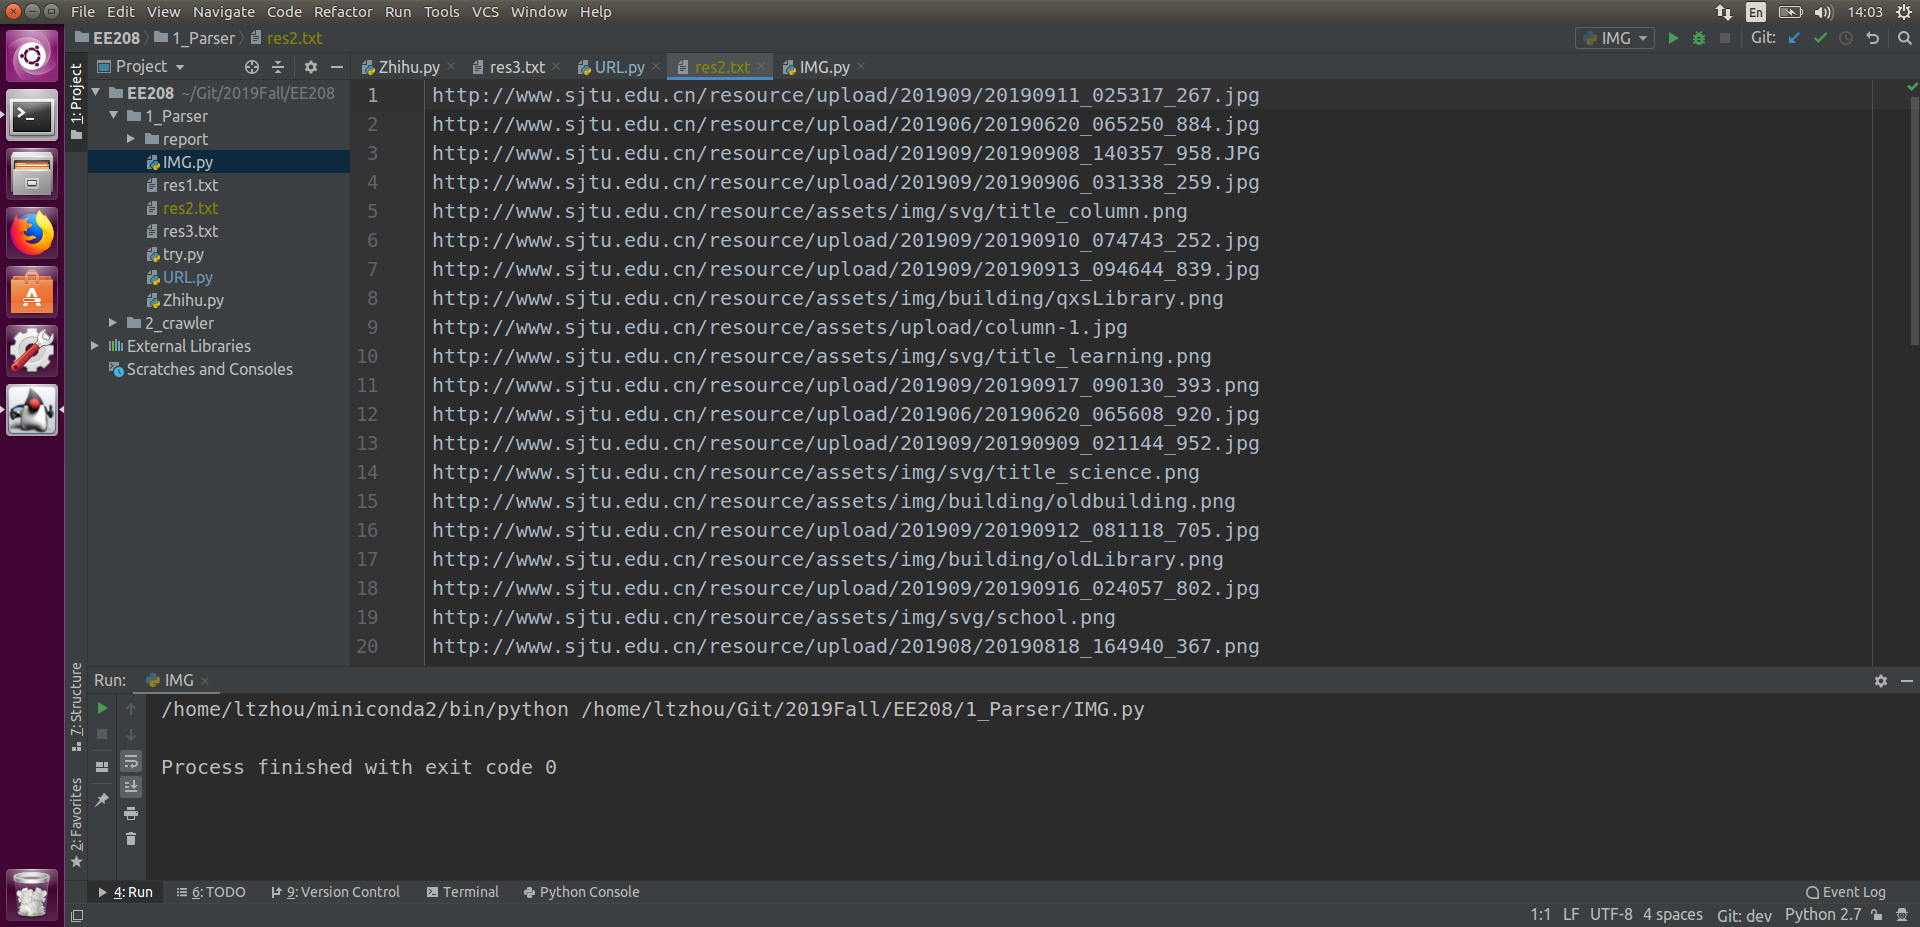
\includegraphics[width=9.5cm]{img/test2_1.png}
\caption{parseIMG in PyCharm}
\label{img:2.1}
\end{figure}

\begin{figure}[htbp]
\centering
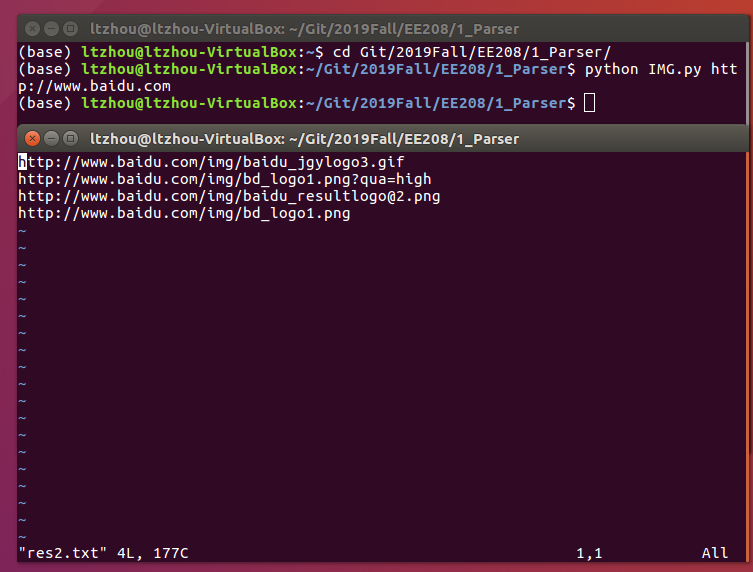
\includegraphics[width=9.5cm]{img/test2_2.png}
\caption{parseIMG in console}
\label{img:2.2}
\end{figure}



\subsection{Exercise 4}

\subsubsection{Solution}

In this exercise we need complete a crawler based on our previous DFS/BFS program. To be more specific, we should implement two concrete functions, namely, get\_page() to get the content of a URL, and get\_all\_links() to get the ChildNodes of a page node.

\paragraph{get\_page()} This function needs to return the page contents of the input URL. Here we require that all the input URLs are in their standard forms. Then with the help of urllib, we can use the built-in read() function to get the page contents. One more thing is done here. We note that the new URLs we've crawled may not be able to visit normally, and that some URLs may point to large files like exe, apk, pdf, etc. In response, a timeout parameter is set here. If it takes too long to visit a URL, the program will automatically abort it. A try-except structure is used here in case of bad URLs.

\begin{python}
# crawler.py
def get_page(page):
    try:
        content = urllib2.urlopen(page,timeout=3).read()
    except:
        print ('Can\'t access to %s' % page)
        content = None
    return content
\end{python}

\paragraph{get\_all\_links()} According to the requirement, we need to extract both the absolute URLs and relative URLs from the `a' label. We use the regular expression given by the hint to implement this idea. The problem here is that we can't just simply put these links into the tocrawl list, since the get\_page function requires standard absolute addresses. Therefore, I wrote another auxiliary function to turn the crawled URL set into a set of standard URLs in the next paragraph.

\begin{python}
# crawler.py
def get_all_links(content,page):
    urlset = set()
    soup = BeautifulSoup(content,features='html.parser')
    for i in soup.findAll('a',{'href': re.compile('^http|^/')}):
        urlset.add(i)
    links = list(URL_set_uniform(urlset,page))
    return links
\end{python}

\paragraph{URL\_set\_uniform()} According to the input URL, three cases are designed. Regular expressions are used to match the relative path, with the urlparse.urljoin() function, relative paths can be transformed into standard URLs. Actually, for the URL regular expression in the previous paragraph, another type of URL will be matched, namely, relative-protocol URL. URL schemes (like http, ftp,...) are omitted in this address. Here we extract the scheme from the original page by urlparse() function, and complete the whole standard URL by adding the scheme at the head of relative-protocol URLs.  

\begin{python}
# crawler.py
def URL_set_uniform(URLset,page):
    urlseg = urlparse.urlparse(page)
    uniURLs = set()
    for i in URLset:
        j = i['href'].split('#')[0]
        if re.match('^//',j):         #case 1: relative-protocol URL
            uniURLs.add(urlseg.scheme+ ':'+j)
        elif (not re.match('://',j)): #case 2: relative path
            uniURLs.add(urlparse.urljoin(page,j))
        else:                         #case 3: standard URL
            uniURLs.add(j)
    return uniURLs
\end{python}




\subsubsection{Results}

In Exercise 4, no parameter in console is required. So whether in IDE or in console, the script will have the same effect. The test results can be found at graph \ref{img:3.1} and \ref{img:3.2}.

\begin{figure}[htbp]
\centering
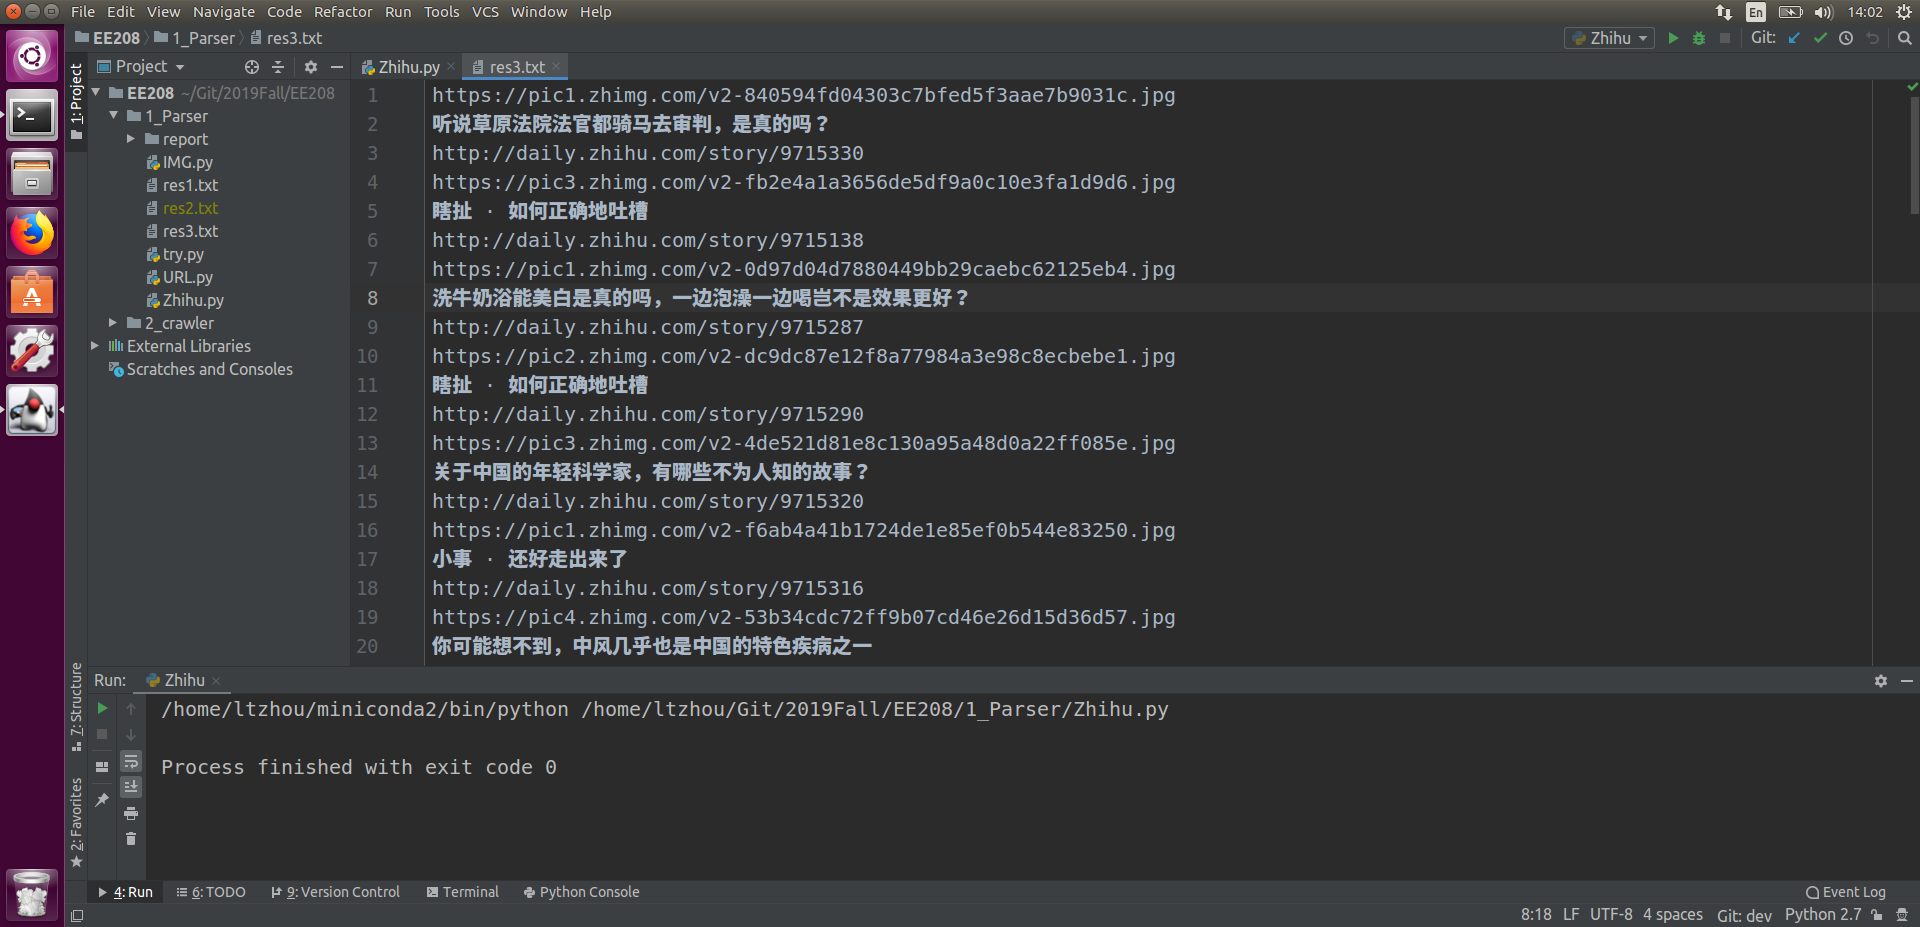
\includegraphics[width=9.5cm]{img/test3_1.png}
\caption{parseZhihuPic in PyCharm}
\label{img:3.1}
\end{figure}

\begin{figure}[htbp]
\centering
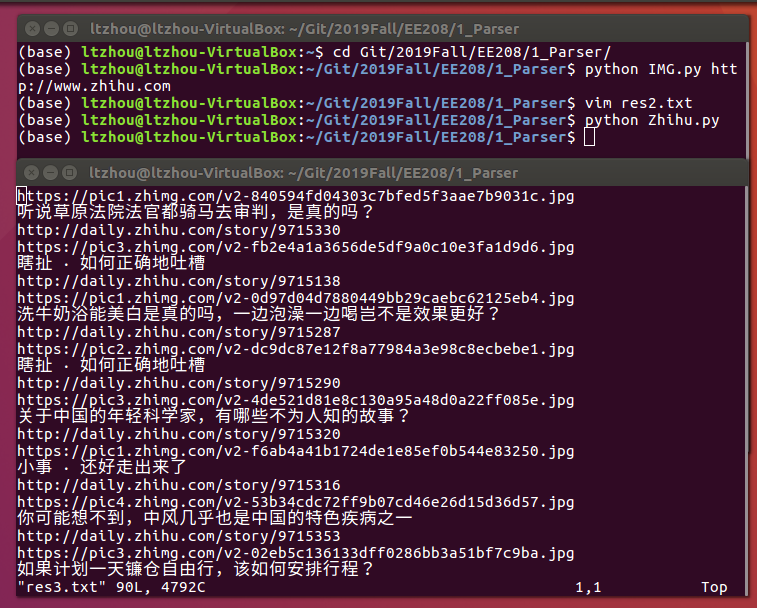
\includegraphics[width=9.5cm]{img/test3_2.png}
\caption{parseZhihuPic in console}
\label{img:3.2}
\end{figure}

\section{Discussion \& Conclusion}
\paragraph{Overview}
Through the practice of this laboratory, I have gained a general knowledge of how the web crawler works and how we can implement DFS, BFS algorithms in the practice of building web crawlers. I've also learnt some web data acquiring skills (such as simulating POST/GET requests) in the course of this lab.

\paragraph{Thoughts}
It has already been known that dividing a big program into several sub-functions will benefit the developing processing a lot. The codes will be a lot easier to read and maintain. Furthermore, after the experiment, I've also learned that it is important to make every part of the small function right. For example, when we're building the crawler, we should pay attention that the link we've crawled should be in the format of standard URL so that the following get\_page() can function well. Only with all things considered, can we work out a reliable program.

\paragraph{Innovations}
In this lab, besides the given function structure, I've written several auxiliary functions for the sake of readability of the program. For example, in Exercise 1, I've divided the whole process into several parts such as cookie initialization, login, and information updating. Another example in Exercise 2 is that I wrote a URL\_set\_uniform function (in fact, copied from my Lab 1) to process the URLs into their standard format. The auxiliary functions can not only simplify our program, they also help make our program more portable to further applications.


\paragraph{Problems \& Solution}
More often than not, Python will report Errors when we are trying to deal with Chinese characters. An efficient way to resolve this issue, as we've done in Lab 1, is to reload the sys module at the beginning of every Python script, as the following codes show. 

\begin{python}
# bbs_set_example.py
import sys
reload(sys)
sys.setdefaultencoding('utf-8')
\end{python}

Another problem in this experiment is that sometimes the URL links we've crawled in a page may not necessary be a website, it can be a document, an exe program or a picture. However, presently, I've not found out an efficient way to eliminate these bad links.  A rough but quick solution, as I've done in Exercise 4, is to add a timeout parameter when we get the contents of the page. Then for large files or ill-connected addresses, Python will report an timeout Error for us to catch and pass. Even if we store some small-sized files that can't be interpreted by HTML parser, it won't take long for the parser to report Error and pass automatically. The problem with this rough solution is that some pages with long HTML scripts or pages that have less satisfactory connection but are still worth crawling will be neglected. I think this issue is still worth attention in the future labs, and I should keep finding appropriate solutions to this problem when furthering my learning.
\begin{python}
# crawler.py
def get_page(page):
    try:
        content = urllib2.urlopen(page,timeout=3).read()
        # a rough solution to bad links
    except:
        print ('Can\'t access to %s' % page)
        content = None
    return content
\end{python}
\end{document}

